\documentclass{beamer}\usepackage[]{graphicx}\usepackage[]{color}
%% maxwidth is the original width if it is less than linewidth
%% otherwise use linewidth (to make sure the graphics do not exceed the margin)
\makeatletter
\def\maxwidth{ %
  \ifdim\Gin@nat@width>\linewidth
    \linewidth
  \else
    \Gin@nat@width
  \fi
}
\makeatother

\definecolor{fgcolor}{rgb}{0.345, 0.345, 0.345}
\newcommand{\hlnum}[1]{\textcolor[rgb]{0.686,0.059,0.569}{#1}}%
\newcommand{\hlstr}[1]{\textcolor[rgb]{0.192,0.494,0.8}{#1}}%
\newcommand{\hlcom}[1]{\textcolor[rgb]{0.678,0.584,0.686}{\textit{#1}}}%
\newcommand{\hlopt}[1]{\textcolor[rgb]{0,0,0}{#1}}%
\newcommand{\hlstd}[1]{\textcolor[rgb]{0.345,0.345,0.345}{#1}}%
\newcommand{\hlkwa}[1]{\textcolor[rgb]{0.161,0.373,0.58}{\textbf{#1}}}%
\newcommand{\hlkwb}[1]{\textcolor[rgb]{0.69,0.353,0.396}{#1}}%
\newcommand{\hlkwc}[1]{\textcolor[rgb]{0.333,0.667,0.333}{#1}}%
\newcommand{\hlkwd}[1]{\textcolor[rgb]{0.737,0.353,0.396}{\textbf{#1}}}%

\usepackage{framed}
\makeatletter
\newenvironment{kframe}{%
 \def\at@end@of@kframe{}%
 \ifinner\ifhmode%
  \def\at@end@of@kframe{\end{minipage}}%
  \begin{minipage}{\columnwidth}%
 \fi\fi%
 \def\FrameCommand##1{\hskip\@totalleftmargin \hskip-\fboxsep
 \colorbox{shadecolor}{##1}\hskip-\fboxsep
     % There is no \\@totalrightmargin, so:
     \hskip-\linewidth \hskip-\@totalleftmargin \hskip\columnwidth}%
 \MakeFramed {\advance\hsize-\width
   \@totalleftmargin\z@ \linewidth\hsize
   \@setminipage}}%
 {\par\unskip\endMakeFramed%
 \at@end@of@kframe}
\makeatother

\definecolor{shadecolor}{rgb}{.97, .97, .97}
\definecolor{messagecolor}{rgb}{0, 0, 0}
\definecolor{warningcolor}{rgb}{1, 0, 1}
\definecolor{errorcolor}{rgb}{1, 0, 0}
\newenvironment{knitrout}{}{} % an empty environment to be redefined in TeX

\usepackage{alltt}

\mode<presentation>
{
  \usetheme{default}      % or try Darmstadt, Madrid, Warsaw, ...
  \usecolortheme{beaver} % or try albatross, beaver, crane, ...
  \usefonttheme{default}  % or try serif, structurebold, ...
  \setbeamertemplate{navigation symbols}{}
  \setbeamertemplate{caption}[numbered]
  \setbeamertemplate{footline}[frame number]
} 

\usepackage[]{natbib}
\usepackage[T1]{fontenc}
\usepackage[english]{babel}

\usepackage{algorithm,algorithmicx,algpseudocode}
\usepackage{amssymb}
 

\usepackage{algorithm}% http://ctan.org/pkg/algorithms
\usepackage{algpseudocode}% http://ctan.org/pkg/algorithmicx

\title{tess3r: a R package for estimating spatial population structure}
\subtitle[\ldots]{Scientific Days, June 13 th \& 14 th , 2017}
\author{Kevin Caye$^{1}$, Olivier Michel$^{2}$, Olivier Francois$^{1}$}
\institute{$^{1}$ TIMC-IMAG, $^{2}$ GIPSA-lab}
\date{}
\titlegraphic{\includegraphics[width=0.2\linewidth]{uga_logo_visuel.jpg}\hspace*{0.2\linewidth}~%
  \includegraphics[width=0.2\linewidth]{persyval.png}\hspace*{0.2\linewidth}~%
  \includegraphics[width=0.2\linewidth]{logoTIMC.jpg}
}
\IfFileExists{upquote.sty}{\usepackage{upquote}}{}
\begin{document}





%%%%%%%%%%%%%%%%%%%%%%%%%%%%%%%%%%%%%%%%%%%%%%%%%%%%%%%%%%%%%%%%%%%%%%%%%%%%%%%%
% TITLE
\frame{\titlepage} 

%%%%%%%%%%%%%%%%%%%%%%%%%%%%%%%%%%%%%%%%%%%%%%%%%%%%%%%%%%%%%%%%%%%%%%%%%%%%%%%%
% Genotypic Data




\begin{frame}{Genotypic Data}
\begin{itemize}
  \item single nucleotide polymorphism (SNP): single nucleotide variation
    occurring commonly within a population.
  \item Data are matrix of size $L$ loci for $n$ individuals ($L \sim 10^6$ and
    $n \sim 10^3$)
\end{itemize}

\begin{center}
\begin{knitrout}
\definecolor{shadecolor}{rgb}{0.969, 0.969, 0.969}\color{fgcolor}
\begin{tabular}{l|r|r|r}
\hline
  & chr: 1 pos: 657 & chr: 1 pos: 3102 & chr: 1 pos: 4648\\
\hline
02B6 & 1 & 1 & 1\\
\hline
09A3 & 1 & 0 & 1\\
\hline
12A1 & 1 & 1 & 1\\
\hline
13B5 & 0 & 0 & 0\\
\hline
\end{tabular}


\end{knitrout}
\end{center}

\end{frame}

%%%%%%%%%%%%%%%%%%%%%%%%%%%%%%%%%%%%%%%%%%%%%%%%%%%%%%%%%%%%%%%%%%%%%%%%%%%%%%%%
% GOAL : Estimating Ancestral Population Structure
\begin{frame}{Goal: Estimating Ancestral Population Structure}

We assume that the genome of each individual come from $K$ ancestral populations. 
We want to estimate: 
\begin{itemize}
  \item \alert{ancestral genotype frequencies} for each locus
  \item \alert{ancestral coefficients} for each individual
\end{itemize}


\includegraphics{barplot.pdf}


Several method exist:
\begin{itemize}
  \item \alert{Bayesian}: structure~\citep{pritchard2000inference}
  \item \alert{optimisation based}: sNMF~\citep{frichot2014fast}
\end{itemize}
These methods are crucial for demographic analysis, medical genetics, 
  conservation genetics or landscape genetics.
\end{frame}

%%%%%%%%%%%%%%%%%%%%%%%%%%%%%%%%%%%%%%%%%%%%%%%%%%%%%%%%%%%%%%%%%%%%%%%%%%%%%%%%
% Spatial Data
\begin{frame}{Spatial Data}

\begin{columns}
\begin{column}{0.5\textwidth}
   %We assume that individuals which are close in space have close ancestry 
   %coefficients. 
Several methods incorporate geographic data in prior distributions:
\begin{itemize}
  \item TESS 2.3~\citep{durand2009spatial}
  \item BAPS~\citep{corander2008bayesian}
\end{itemize}

\end{column}
\begin{column}{0.5\textwidth}  %%<--- here
    \begin{center}
    \includegraphics{map.pdf}
     \end{center}
\end{column}
\end{columns}
We propose a new method to estimate spatial population based on an optimizarion 
problem.
\end{frame}

%%%%%%%%%%%%%%%%%%%%%%%%%%%%%%%%%%%%%%%%%%%%%%%%%%%%%%%%%%%%%%%%%%%%%%%%%%%%%%%%
% MODEL SNMF
\begin{frame}{Model for the Genotypic Matrix}

We write $G$ the genomic matrix

\begin{equation*}
\begin{array}{rcl}
P(G_{i,\ell} = j) & = & \sum_{k=1}^K Q_{i,k} f_{k,\ell}(j),\\
\\
P &=& QF^T,
\end{array}
\end{equation*}

where $Q$ is the ancestry coefficient matrix and $F$ the ancestral genotype 
frequency matrix. There are such as: 

\begin{equation*}
\begin{aligned}
Q \succeq 0,~\sum_{k=1}^{K} Q_{i,k} = 1,~\forall i \in \{1,...,n\}  \\
F \succeq 0,~\sum_{j=0}^{d} f_{k,\ell}(j) = 1,~\forall \ell \in \{1,...,L\}.
\end{aligned}
\end{equation*}

\end{frame}

%%%%%%%%%%%%%%%%%%%%%%%%%%%%%%%%%%%%%%%%%%%%%%%%%%%%%%%%%%%%%%%%%%%%%%%%%%%%%%%%
% OPTIM PB

\begin{frame}{Optimisation Problem}

We construct a weighted graph using spatial data:

\begin{equation*}
W_{i,j} = e^{ - \frac{||z_i - z_j||^2}{\sigma}},
\end{equation*}

where $z$ are geographic positions.

The loss function is:

\begin{equation*}
\begin{aligned}
Loss(Q,F)& = &||X-QF^T||^2 + \lambda \sum_{i,j}^{n} W_{i,j} ||Q_{i,} - Q_{j,}||^2 \\
 &= &||X-QF^T||^2 + \lambda \text{trace}(Q^T \Lambda Q),
\end{aligned}
\end{equation*}

where $\Lambda$ is the graph Laplacian matrix and $X$ is the data matrix.
% is a binary matrix which encode absence or the presence of each genotype at each locus.

\end{frame}

%%%%%%%%%%%%%%%%%%%%%%%%%%%%%%%%%%%%%%%%%%%%%%%%%%%%%%%%%%%%%%%%%%%%%%%%%%%%%%%%
% ALGO

\begin{frame}{Block-coordinate Descent Scheme}

\begin{itemize}

\item The optimisation problem is not convex.

\item It is convex with respect to one of the variables $Q$ or $F$ when the other one is fixed.

\item We can use a block-coordinate descent scheme:

\begin{algorithmic}
\For {$it \in {1,..,itMax}$}

$ F \gets \underset{F}{\text{arg min}} f_F(Q,F)$

$ Q \gets \underset{Q}{\text{arg min}} f_Q(Q,F)$

\EndFor
\end{algorithmic}

\end{itemize}

\end{frame}

%%%%%%%%%%%%%%%%%%%%%%%%%%%%%%%%%%%%%%%%%%%%%%%%%%%%%%%%%%%%%%%%%%%%%%%%%%%%%%%%

\begin{frame}{Alternating Projected Least Squares}

F optimisation step : 
\begin{enumerate}
  \item Solving least squares problems for $F$ rows
  \item Projecting onto the polygon of $F$ constraints
\end{enumerate}
Q optimisation step : 
\begin{enumerate}
  \item Solving $L_2$-regularized least squares problems for $Q$ rows
  \item Projecting onto the polygon of $Q$ constraints
\end{enumerate}

\end{frame}

%%%%%%%%%%%%%%%%%%%%%%%%%%%%%%%%%%%%%%%%%%%%%%%%%%%%%%%%%%%%%%%%%%%%%%%%%%%%%%%%

\begin{frame}{Alternating Projected Least Squares}

\begin{itemize}

\item Advantage:

The $F$ optimisation step requires to solve $L$ least squares problems of size $K$.

The $Q$ optimisation step requires to solve $n$ $L_2$-regularized least squares problems of size $K$.

\item Drawback:

The algorithm is not guaranteed to provide a stationary point.

\end{itemize}

\end{frame}

%%%%%%%%%%%%%%%%%%%%%%%%%%%%%%%%%%%%%%%%%%%%%%%%%%%%%%%%%%%%%%%%%%%%%%%%%%%%%%%%
% Numerical experiement 2 slides présentation de l'experimentation + resultats
\begin{frame}{Simulations}

Simulation of admixed population dataset~\citep{franccois2010spatially}
\begin{center}
\includegraphics[width=.70\linewidth]{addmixed.png}
\end{center}

\end{frame}

%%%%%%%%%%%%%%%%%%%%%%%%%%%%%%%%%%%%%%%%%%%%%%%%%%%%%%%%%%%%%%%%%%%%%%%%%%%%%%%%

\begin{frame}{Comparison with TESS 2.3 }
On these simulation TESS3 algorithm performs 30 time better than TESS 2.3

\begin{figure}[h!]\centering
\begin{minipage}{0.49\textwidth}
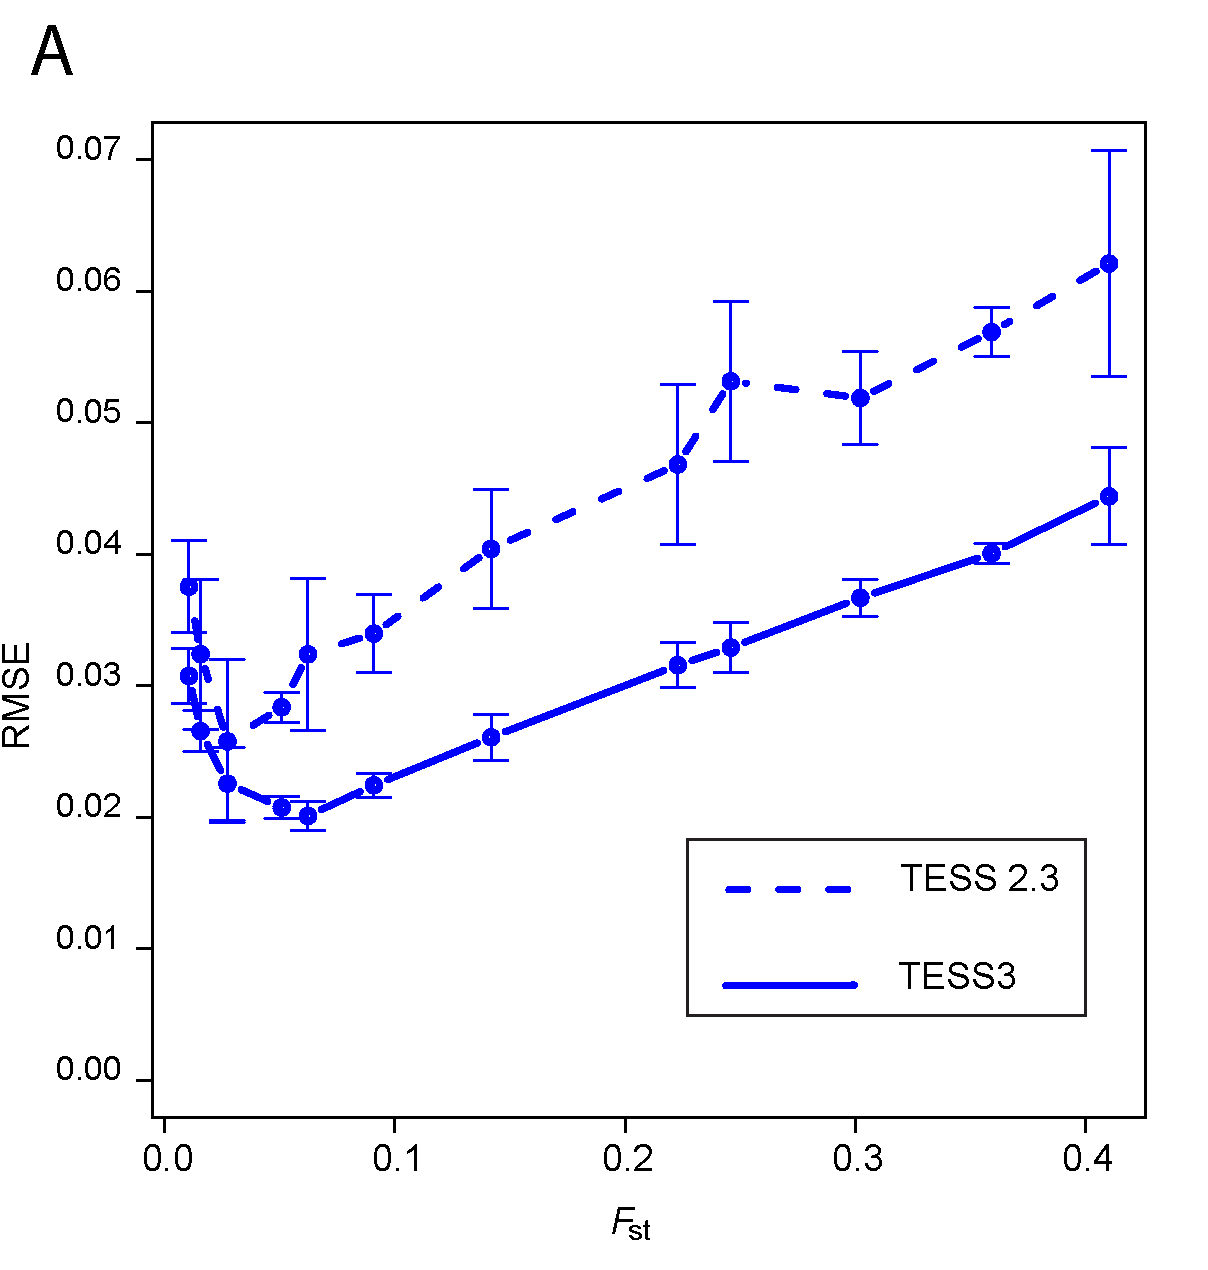
\includegraphics[width=\linewidth]{rmseG.pdf}
\end{minipage}
\begin {minipage}{0.49\textwidth}
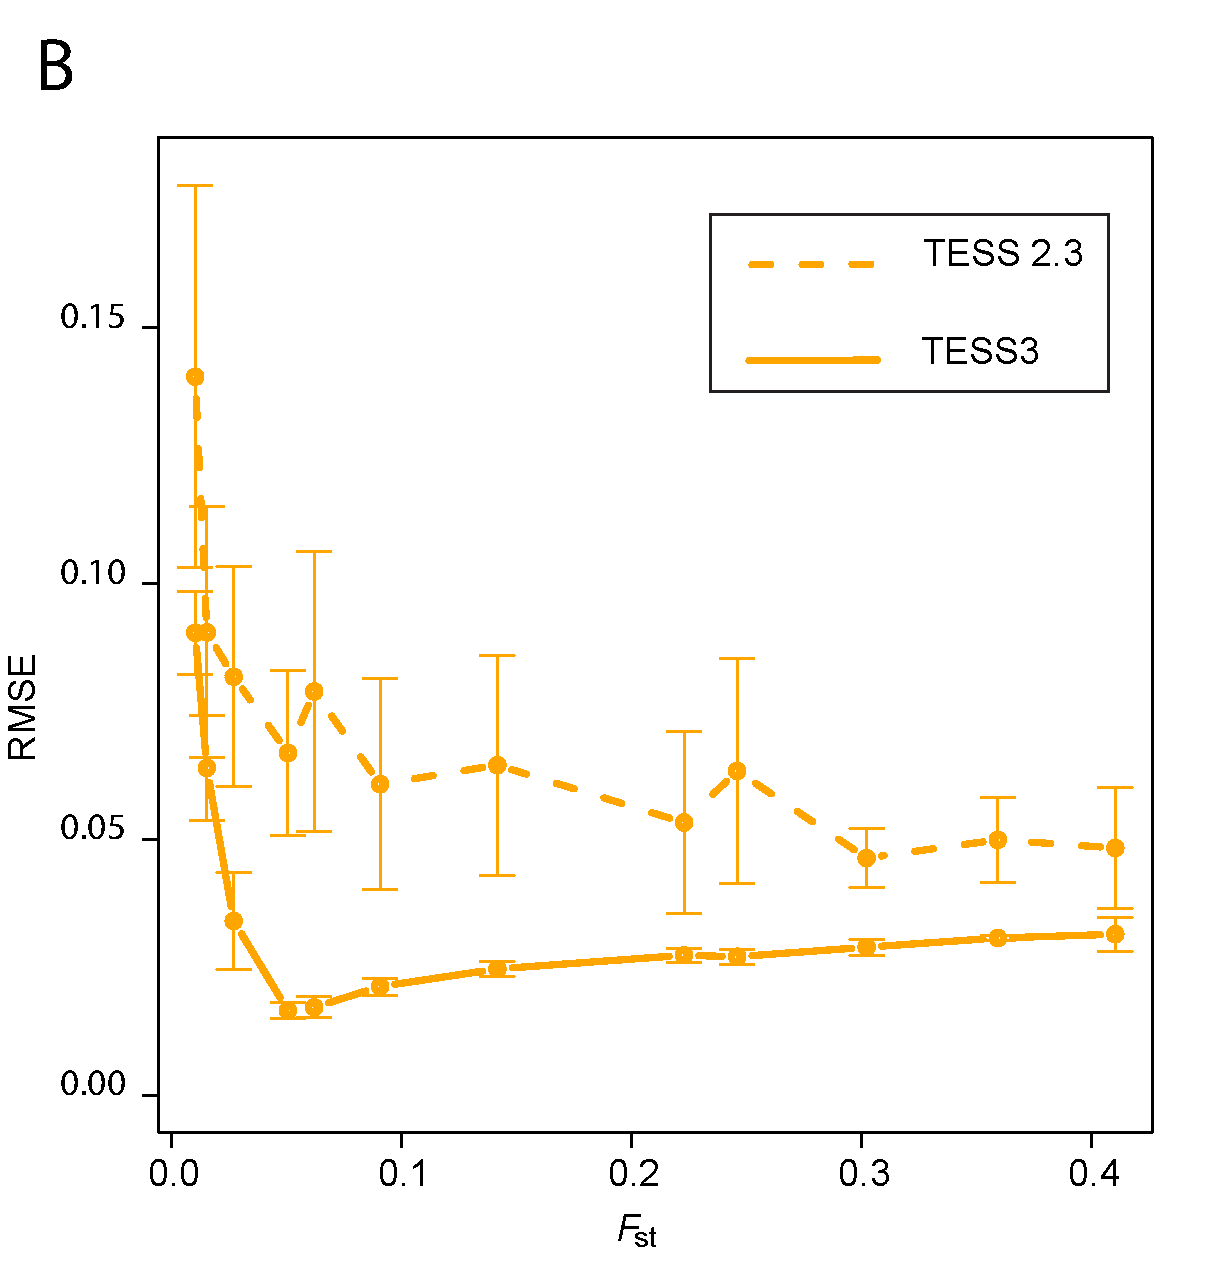
\includegraphics[width=\linewidth]{rmseQ.pdf}
\end{minipage}
\caption{A) RMSEs of $F$ estimates. B) RMSEs of $Q$ estimates.}
\end{figure}

\end{frame}

%%%%%%%%%%%%%%%%%%%%%%%%%%%%%%%%%%%%%%%%%%%%%%%%%%%%%%%%%%%%%%%%%%%%%%%%%%%%%%%%
% ARABIDOPSIS THALIANA : Data
\begin{frame}{\emph{Arabidopsis thaliana} RegMap Lines Dataset}

\begin{figure}[H]
   \includegraphics[width=0.45\linewidth]{a_thaliana.jpg}
  \label{fig:ma_fig}

\end{figure}

\begin{itemize}
  \item 1,307 accessions of \emph{A. thaliana} have been genotyped using the Affymetrix Arabidopsis 250k - SNP chip~\citep{horton2012genome}
  \item Geographic coordinates for 1,193 of these samples~\citep{anastasio2011source}
\end{itemize}

\end{frame}

%%%%%%%%%%%%%%%%%%%%%%%%%%%%%%%%%%%%%%%%%%%%%%%%%%%%%%%%%%%%%%%%%%%%%%%%%%%%%%%%
% ARABIDOPSIS THALIANA : K = 3

\begin{frame}{Ancestry Coefficients with $K = 3$ Ancestral Populations}
\begin{center}
\includegraphics[width=0.9\linewidth]{Q_K3.pdf}
\end{center}
\end{frame}

%%%%%%%%%%%%%%%%%%%%%%%%%%%%%%%%%%%%%%%%%%%%%%%%%%%%%%%%%%%%%%%%%%%%%%%%%%%%%%%%
% ARABIDOPSIS THALIANA : rmse X K

\begin{frame}{Selection of the Number of Ancestral Populations}
We choose \alert{$K = 6$} ancestral populations.

\begin{center}
\includegraphics{KSelection.pdf}
\end{center}

\end{frame}

%%%%%%%%%%%%%%%%%%%%%%%%%%%%%%%%%%%%%%%%%%%%%%%%%%%%%%%%%%%%%%%%%%%%%%%%%%%%%%%%
% ARABIDOPSIS THALIANA : variogramme

\begin{frame}{Selection of the Spatial Autocorrelation Scale}
We choose \alert{$\sigma = 1.5$} for the spatial autocorrelation scale.
\begin{center}
\includegraphics{variogram.pdf}
\end{center}

\end{frame}

%%%%%%%%%%%%%%%%%%%%%%%%%%%%%%%%%%%%%%%%%%%%%%%%%%%%%%%%%%%%%%%%%%%%%%%%%%%%%%%%
% ARABIDOPSIS THALIANA : K = 6 et sigma = 1.5

\begin{frame}{Ancestry Coefficients for $K = 6$ and $\sigma = 1.5$}
\begin{center}
\includegraphics{Q_K6_sigma1_5.pdf}
\end{center}
\end{frame}

%%%%%%%%%%%%%%%%%%%%%%%%%%%%%%%%%%%%%%%%%%%%%%%%%%%%%%%%%%%%%%%%%%%%%%%%%%%%%%%%
% ARABIDOPSIS THALIANA : manhattan plot

\begin{frame}{Ancestral Frequency Manhattan Plot for $K = 6$ and $\sigma = 1.5$}
\begin{center}
\includegraphics{G_K6_sigma1_5.png}
\end{center}
\end{frame}

%%%%%%%%%%%%%%%%%%%%%%%%%%%%%%%%%%%%%%%%%%%%%%%%%%%%%%%%%%%%%%%%%%%%%%%%%%%%%%%%

\begin{frame}{Detecting Adaptive Loci (Preliminary Results)}
\begin{itemize}
  \item Flowering-related genes detected in the top list: FRIGIDA, FLOWERING LOCUS C (FLC), 
  DELAY OF GERMINATION 1 (DOG1)~\citep{horton2012genome}.
  \item Statistical overrepresentation of genes involved in metabolic processes: 
  1.08 fold enrichment, $p$-value $< 1e^{-6}$ (PANTHER database).
\end{itemize}
  
\end{frame}


%%%%%%%%%%%%%%%%%%%%%%%%%%%%%%%%%%%%%%%%%%%%%%%%%%%%%%%%%%%%%%%%%%%%%%%%%%%%%%%%
% Conclusion: (résumé) 

\begin{frame}[fragile]{Conclusion}

\begin{itemize}
  \item Estimation and visualisation of spatial population structure.
  \item Local adaptation detection.
  \item Beta Version available on github.

\end{itemize}

  
\begin{knitrout}
\definecolor{shadecolor}{rgb}{0.969, 0.969, 0.969}\color{fgcolor}\begin{kframe}
\begin{alltt}
\hlstd{devtools}\hlopt{::}\hlkwd{install_github}\hlstd{(}\hlstr{"cayek/TESS3_encho_sen@master"}\hlstd{)}
\end{alltt}
\end{kframe}
\end{knitrout}

\end{frame}

%%%%%%%%%%%%%%%%%%%%%%%%%%%%%%%%%%%%%%%%%%%%%%%%%%%%%%%%%%%%%%%%%%%%%%%%%%%%%%%%
% Thanks

\begin{frame}{Acknowledgments}
\begin{itemize}
  \item Timo Deist, Eric Frichot, Olivier Fran\c cois, Olivier Michel 
  \item This Ph.D is funded by the labex Persyval-lab
\end{itemize}

\begin{center}
\Huge \alert{Thank you for your attention.}
\end{center}

\end{frame}

%%%%%%%%%%%%%%%%%%%%%%%%%%%%%%%%%%%%%%%%%%%%%%%%%%%%%%%%%%%%%%%%%%%%%%%%%%%%%%%%
% %\section{Study of \protect\emph{Arabidopsis thaliana} with tess3r}
%%%%%%%%%%%%%%%%%%%%%%%%%%%%%%%%%%%%%%%%%%%%%%%%%%%%%%%%%%%%%%%%%%%%%%%%%%%%%%%%
% ARABIDOPSIS THALIANA : Data
% 
% \begin{frame}{\emph{Arabidopsis thaliana} RegMap lines~\citep{horton2012genome} dataset}
% 
% - pres data
% 
% \end{frame}
% 
% - avec K = 3
% - choix de K
% - chois de sigma
% - K = 6
% - manhattan plot + quelques gènes
% - manhattan plot + fdr
% - étude de sur représentation
% 
% \begin{frame}{Ancestry Coefficient Matrix With $K = 3$ Ancestral Population}
% 
% \frame{frame}
% 
% %%%%%%%%%%%%%%%%%%%%%%%%%%%%%%%%%%%%%%%%%%%%%%%%%%%%%%%%%%%%%%%%%%%%%%%%%%%%%%%%
% % CONCLUSION en faite pas util...
% % \begin{frame}{Conclusion}
% % \begin{itemize}
% % \imetize Optimization based model for estimating spatial population structure.
% % \imetize A R package implementation which can be use in a R workflow.
% % \imetize A R package for estimation and visualisation.
% % \begin{end}
% % \end{frame}
% %%%%%%%%%%%%%%%%%%%%%%%%%%%%%%%%%%%%%%%%%%%%%%%%%%%%%%%%%%%%%%%%%%%%%%%%%%%%%%%%
% % % REF and THANKS
%\begin{frame}{References}
 
\bibliographystyle{plainnat}
\bibliography{main}
 
%\end{frame}

\end{document}

